\begin{frame}[fragile,label=HTMLForms1]{HTML forms (1)}
\begin{minted}[fontsize=\small]{HTML}
<form action="https://example.com/search/" method="GET">
<input type="hidden" name="recipient"
       value="webmaster@example.com">
Search for: <input name="q" value=""><br>
<input type="submit" value="Search">
</form>
\end{minted}
\hrule
    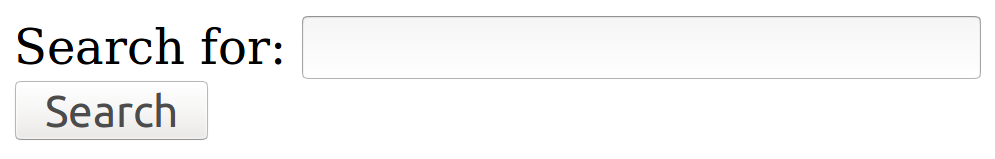
\includegraphics[width=\textwidth]{form1-rendered}
\end{frame}

\begin{frame}[fragile,label=HTMLForms2]{HTML forms (2)
\begin{framed}
\tt\small
GET /search/?q=What\%20I\%20searched\%20for HTTP/1.1 \\
Host: example.com
\end{framed}
    \begin{itemize}
        \item q is ``\fbox{What I searched for}''
        \item \%20 --- character hexadecimal 20 (space)
    \end{itemize}
\end{frame}

\begin{frame}[fragile,label=HTMLForms3]{HTML forms (3)}
\begin{minted}[fontsize=\small]{HTML}
<form action="https://example.com/formmail.pl" method="POST">
<input type="hidden" name="recipient"
       value="webmaster@example.com">
Your email: <input name="from" value=""><br>
Your message:<textarea name="message"></textarea>
<input type="submit">
</form>
\end{minted}
\begin{framed}
\tt\small
POST /formmail.pl HTTP/1.1 \\
Host: example.com \\
Content-Type: application/x-www-form-urlencoded \\
~ \\
recipient=webmaster@example.com\&from=\textit{what\%20I\%20Entered}\\\&message=\textit{Some\%20message\%0a\ldots} \\
\end{framed}
\end{frame}


